% Short report, Assignment 2a: forced alignment with the Montreal Forced Aligner
% Build (from this folder): xelatex report.tex  (run twice)
\documentclass[11pt,a4paper]{article}
\usepackage{fontspec}
\usepackage[margin=2.0cm]{geometry}
\usepackage{graphicx,booktabs,caption,enumitem,float,tabularx}
\usepackage[hidelinks]{hyperref}
\setmainfont{Cambria}
\setmonofont{Consolas}[Scale=0.86]
\newfontfamily\ipa{Segoe UI}
\newcommand{\code}[1]{\texttt{#1}}
\graphicspath{{../outputs/figures/}{figures/}}
\setlist{itemsep=1pt,topsep=3pt}
\captionsetup{font=small,labelfont=bf}
\setlength{\parskip}{3pt}
\emergencystretch=2em
\renewcommand{\floatpagefraction}{0.85}
\renewcommand{\topfraction}{0.85}

\title{Forced alignment with the Montreal Forced Aligner,\\ and the aligner as a pronunciation checker\\[3pt]\large Assignment 2a report}
\author{Simhaa T.\,T.}
\date{November 2026}

\begin{document}
\maketitle

\section{Summary}
Forced alignment finds when each word and each speech sound (phone) of a known transcript starts and ends in a
recording. The six provided recordings are three news readings of 25--31\,s and three 4-second clips of a
non-native speaker saying minimal pairs (``I said BAD not BED''). I aligned them with the Montreal Forced Aligner
(MFA) 3.4.3 in four setups, which combine two acoustic models, pretrained or extended pronunciation dictionaries
and, once, recordings with the trailing silence cut (Table~\ref{tab:setups}). One command,
\code{python run\_pipeline.py}, runs every step.

The two acoustic models put the same word boundary within 20\,ms of each other for 90\% of the 488 word
boundaries, and within 10\,ms at the median. Pronunciations generated for the five unknown-word tokens gave them
real phones and moved no other boundary by more than 20\,ms. The clearest error comes from \code{english\_mfa}: in
two of the three short clips it stretched a word-final stop over the trailing silence, so ``bed'' lasts 3.0\,s
instead of 0.55\,s. Cutting the trailing silence caps the largest disagreement at 0.25\,s but does not cure the
error.

Plain forced alignment cannot notice a mispronunciation: it labels the non-native speaker's ``bad'' and ``bed''
/æ/ and /ɛ/ because the dictionary says so. I therefore also used the aligner as a pronunciation checker, letting
the acoustic model choose between each word's own vowel and its partner's. It chose the vowel of ``bed'' for
``bad'', and ``bad'' is the only one of six words whose partner vowel fits the audio better. The formants point the
same way: this speaker's ``bad'' lies between /æ/ and /ɛ/.

\section{Data and preparation}
Figure~\ref{fig:pipeline} shows the five steps of the pipeline, from the provided files to the analysis.

\begin{figure}[!tbp]\centering
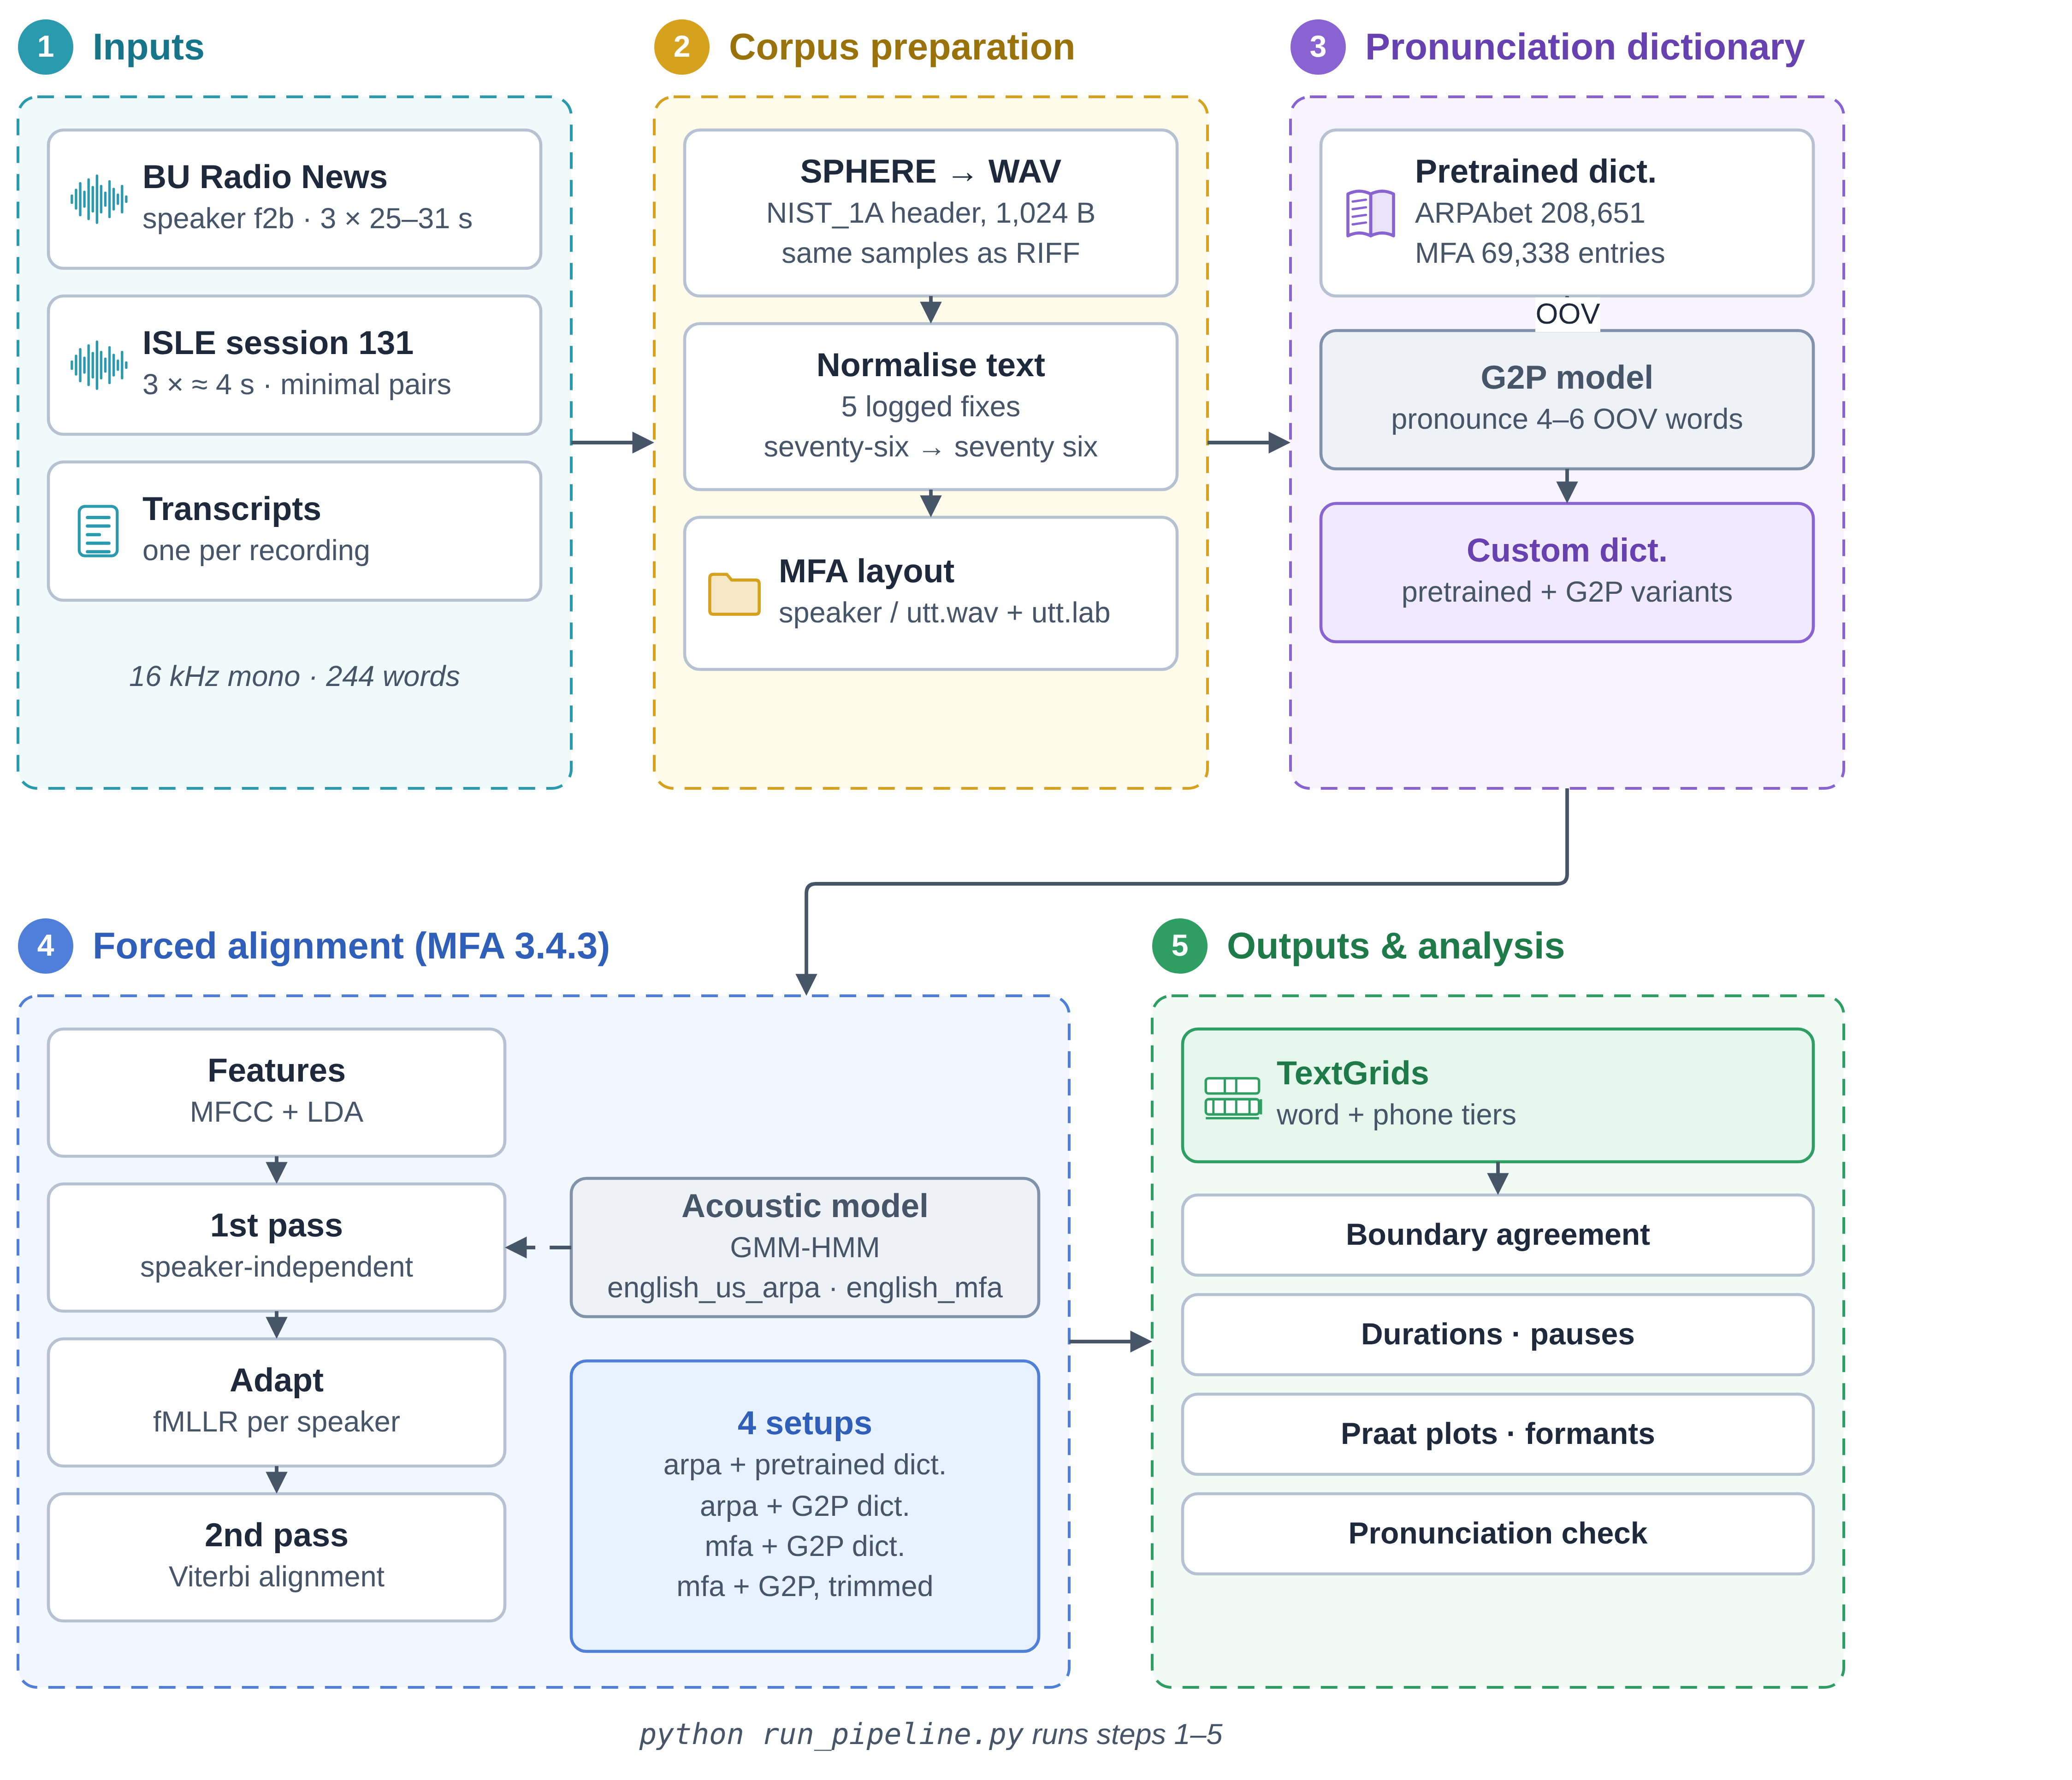
\includegraphics[width=0.86\linewidth]{fig1_pipeline.png}
\caption{The pipeline. The script converts the audio and cleans the transcripts, generates pronunciations for
unknown words (OOV, out of vocabulary), aligns every file in four setups and analyses the TextGrids.}
\label{fig:pipeline}
\end{figure}

\begin{table}[H]\centering\small
\caption{The provided recordings (16\,kHz, mono).}
\label{tab:data}
\begin{tabularx}{\linewidth}{@{}llrr>{\raggedright\arraybackslash}X@{}}
\toprule
Files & Speaker & Length & Words & Content \\
\midrule
\code{F2BJRLP1}--\code{3} & BU Radio News f2b, female & 25--31\,s & 73, 73, 82 & read news story \\
\code{ISLE\_\ldots\_01}--\code{03} & ISLE session 131, male & 3.9--4.5\,s & 5 each &
``I said X not Y'' minimal pairs \\
\bottomrule
\end{tabularx}
\end{table}

MFA expects one folder per speaker holding \code{<utterance>.wav} and a transcript \code{<utterance>.lab} with the
same name (\code{scripts/prepare\_corpus.py}). Before that, I fixed two problems in the provided data.
\begin{itemize}
\item \textbf{The news files are not WAV files.} \code{F2BJRLP*.wav} start with the header \code{NIST\_1A}: they are
NIST SPHERE files with a \code{.wav} name. The script reads the 1,024-byte header (16-bit little-endian PCM,
16\,kHz) and rewrites the same samples as RIFF WAV.
\item \textbf{The news transcripts contain tokens nobody says as written.} The script joins the lines and makes
five changes, logged in \code{outputs/corpus/normalisation\_log.tsv}. Three repair numbers split across a line
(\emph{seventy- six} $\to$ \emph{seventy six}); two spell out letters that the reader says one by one
(\emph{S.J.C.'s} $\to$ \emph{S J C's}, \emph{WBUR's} $\to$ \emph{W B U R's}).
\end{itemize}

\section{Models and dictionaries}
\begin{table}[H]\centering\small
\caption{The four alignment setups; the first is \code{english\_us\_arpa\_pretrained\_dict} in the outputs. Both
acoustic models are GMM-HMMs on LDA-transformed MFCC features, trained by the MFA developers; MFA runs a
speaker-independent pass, adapts to each speaker (fMLLR) and aligns again.}
\label{tab:setups}
\begin{tabularx}{\linewidth}{@{}lll>{\raggedright\arraybackslash}X@{}}
\toprule
Setup & Acoustic model & Phone set & Dictionary \\
\midrule
\code{\ldots\_pretrained\_dict} & \code{english\_us\_arpa} (MFA 3.0) & ARPAbet & pretrained
\code{english\_us\_arpa}, 208,651 entries \\
\code{english\_us\_arpa} & \code{english\_us\_arpa} (MFA 3.0) & ARPAbet & the same + G2P for 4 words \\
\code{english\_mfa} & \code{english\_mfa} (MFA 3.1) & IPA-based & pretrained \code{english\_us\_mfa},
69,338 entries, + G2P for 6 words \\
\code{english\_mfa\_trimmed} & \code{english\_mfa} (MFA 3.1) & IPA-based & the same; trailing silence cut
(Section~\ref{sec:obs}) \\
\bottomrule
\end{tabularx}
\end{table}

\paragraph{Custom dictionary.} \code{mfa g2p} with \code{--dictionary\_path} generates pronunciations only for
words missing from the given dictionary. The ARPAbet dictionary lacks four: \emph{Dukakis}, \emph{Maffy},
\emph{Melnicove} and \emph{politicize} (MFA splits \emph{de-politicize} at the hyphen, and \emph{de} is known). The
MFA dictionary also lacks \emph{Margo} and \emph{judgeships}. For uncertain names G2P returns several variants,
five for \emph{Dukakis}, and the aligner picks the one that fits the audio best: \code{D UW1 K AA1 K IH0 S}
with ARPAbet, and the reduced {\ipa d ɐ k ə c ɪ s} with the MFA phone set. Figure~\ref{fig:setups} shows how the
models and dictionaries combine into the four setups.

\begin{figure}[!tbp]\centering
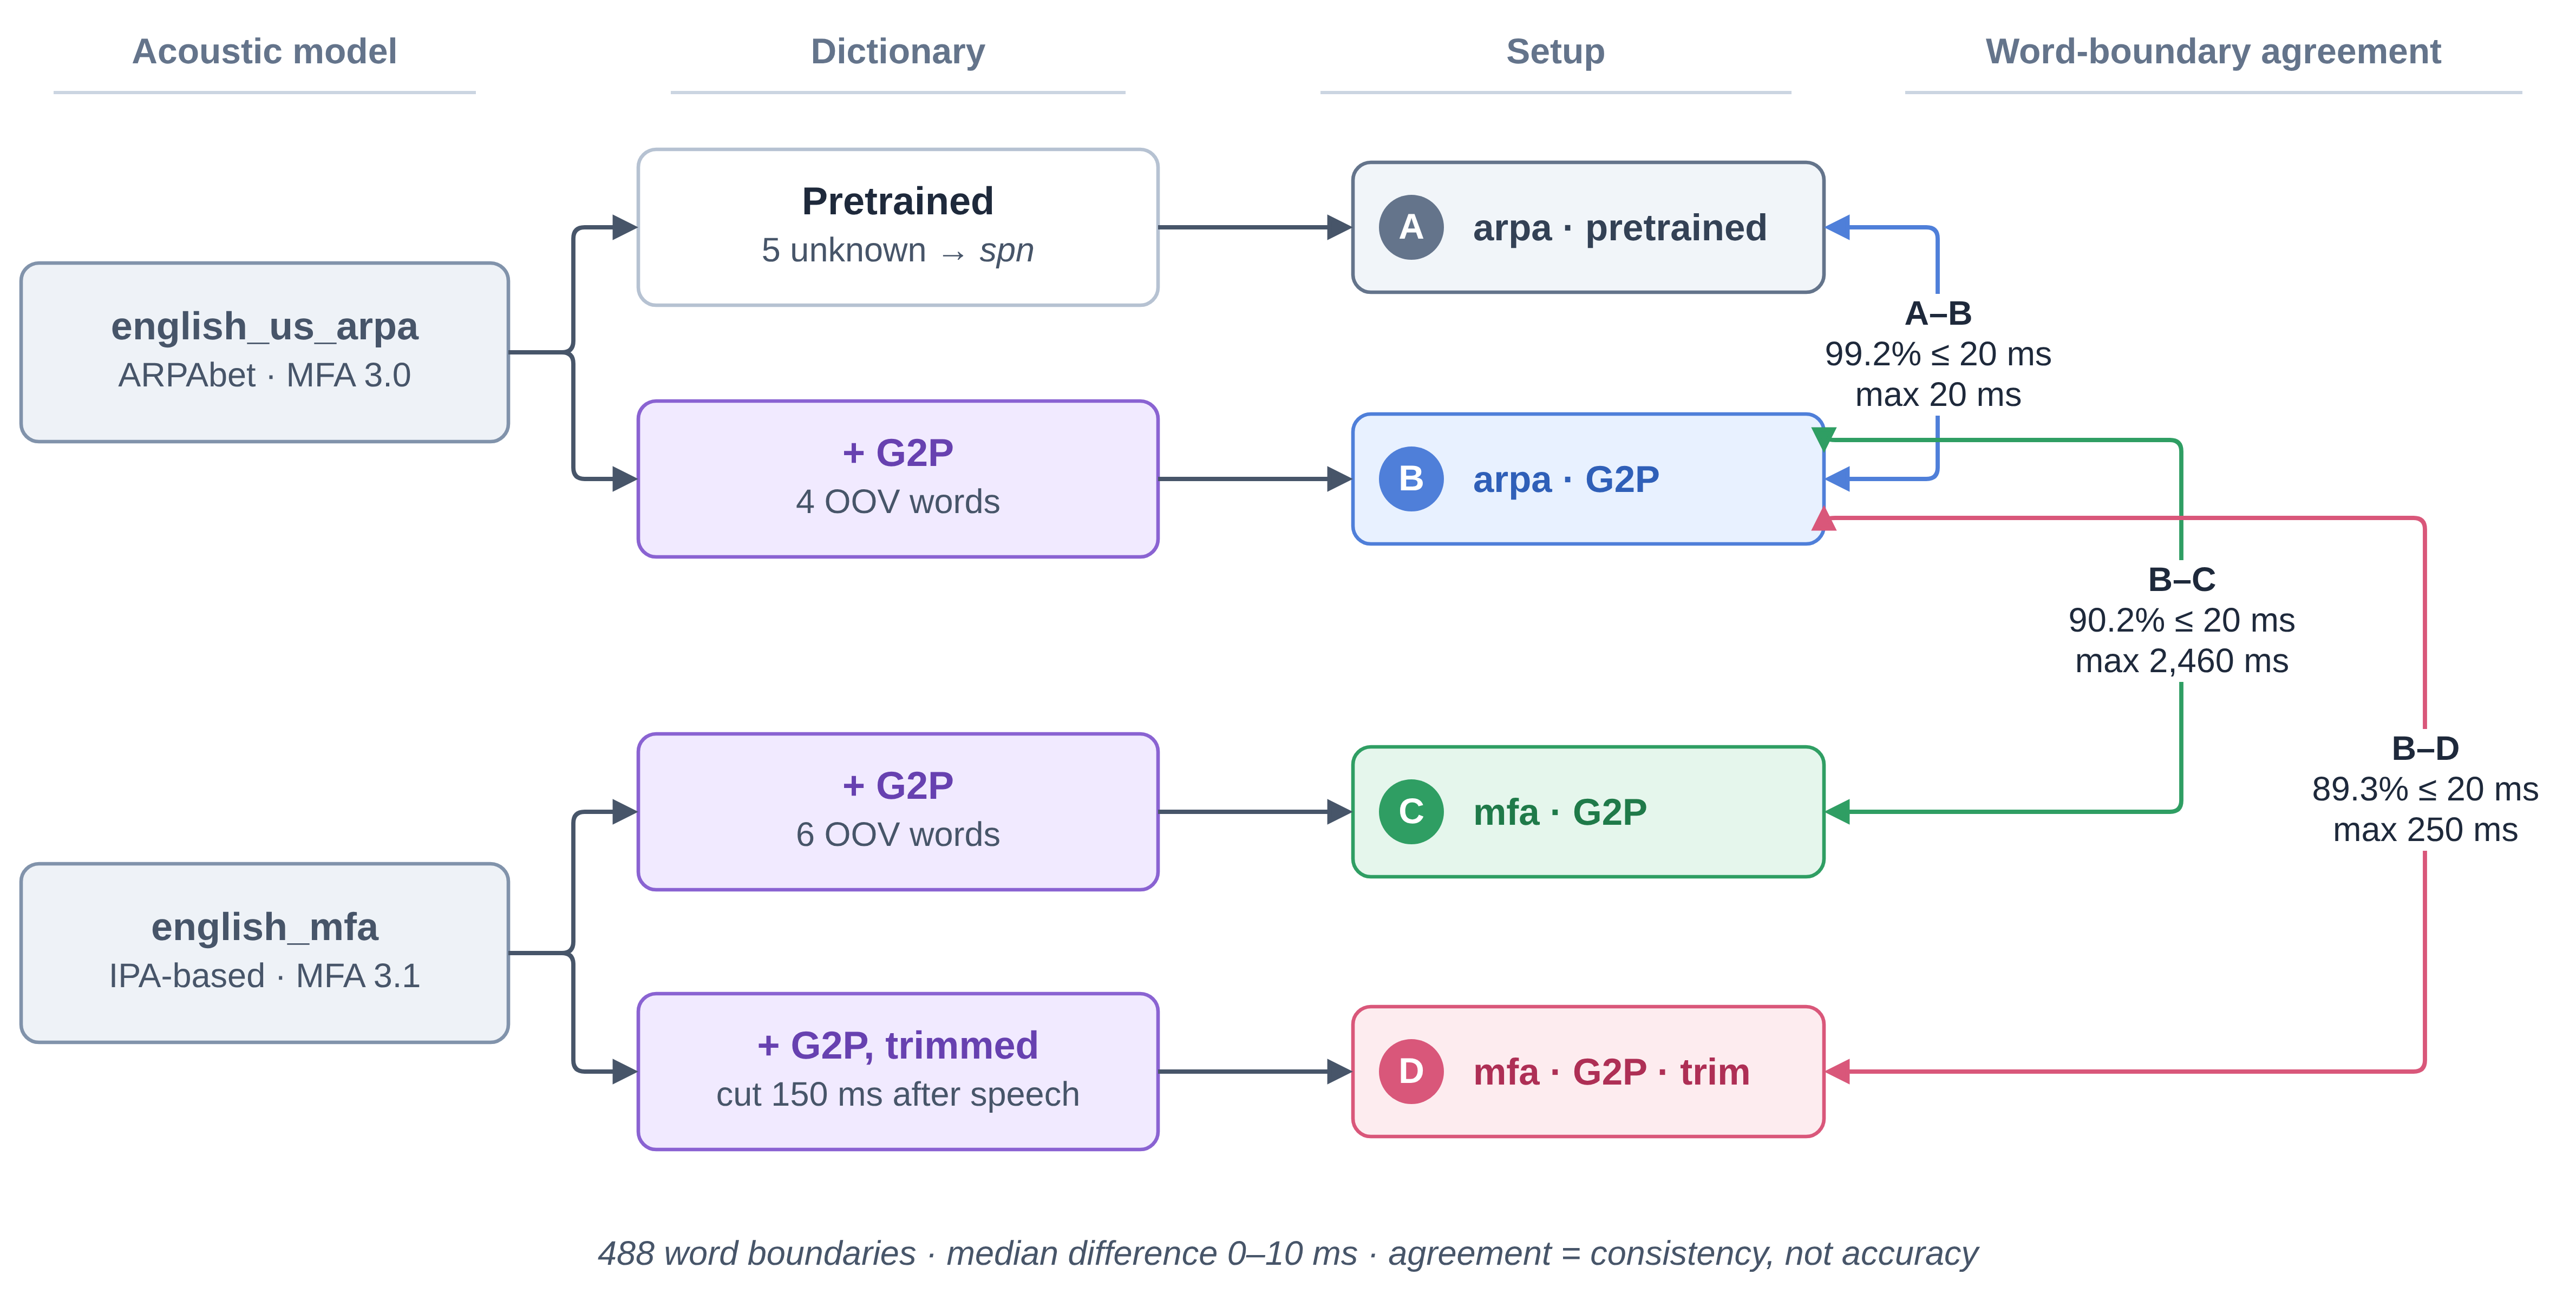
\includegraphics[width=0.92\linewidth]{fig2_setups_agreement.png}
\caption{How the four setups (A--D) arise from two acoustic models and three dictionaries, and how often their
word boundaries agree within 20\,ms (Table~\ref{tab:agree}). Setup B serves as the reference for the others.}
\label{fig:setups}
\end{figure}

\section{Results}
\begin{table}[H]\centering\small
\caption{What each setup produced over all six files (244 words). ``Unknown'' words get the single filler phone
\code{spn} instead of phones. ``Median'' is the median phone duration; ``$\leq$ 30\,ms'' counts phones of three
frames or fewer.}
\label{tab:summary}
\begin{tabular}{@{}lrrrrr@{}}
\toprule
Setup & Unknown words & Phones & Median & $\leq$ 30\,ms & Pauses $\geq$ 100\,ms \\
\midrule
\code{english\_us\_arpa}, pretrained dict. & 5 & 1,028 & 70\,ms & 78 & 22 \\
\code{english\_us\_arpa} (G2P) & 0 & 1,063 & 70\,ms & 82 & 22 \\
\code{english\_mfa} (G2P) & 0 & 1,045 & 70\,ms & 96 & 19 \\
\code{english\_mfa\_trimmed} (G2P) & 0 & 1,045 & 70\,ms & 98 & 19 \\
\bottomrule
\end{tabular}
\end{table}

\begin{table}[H]\centering\small
\caption{Agreement of word boundaries between setups (start and end of all 244 words, 488 boundaries). With no
hand-made reference alignment, agreement shows consistency, not accuracy.}
\label{tab:agree}
\begin{tabular}{@{}lrrrr@{}}
\toprule
Setups compared & Median diff. & Within 20\,ms & Within 50\,ms & Largest \\
\midrule
\code{english\_us\_arpa} vs \code{english\_mfa} & 10\,ms & 90.2\% & 96.3\% & 2,460\,ms (``bed'') \\
\code{english\_us\_arpa} vs \code{english\_mfa\_trimmed} & 10\,ms & 89.3\% & 96.1\% & 250\,ms (``he'') \\
\code{english\_us\_arpa}, pretrained vs G2P dict. & 0\,ms & 99.2\% & 100\% & 20\,ms \\
\bottomrule
\end{tabular}
\end{table}

\begin{figure}[!tbp]\centering
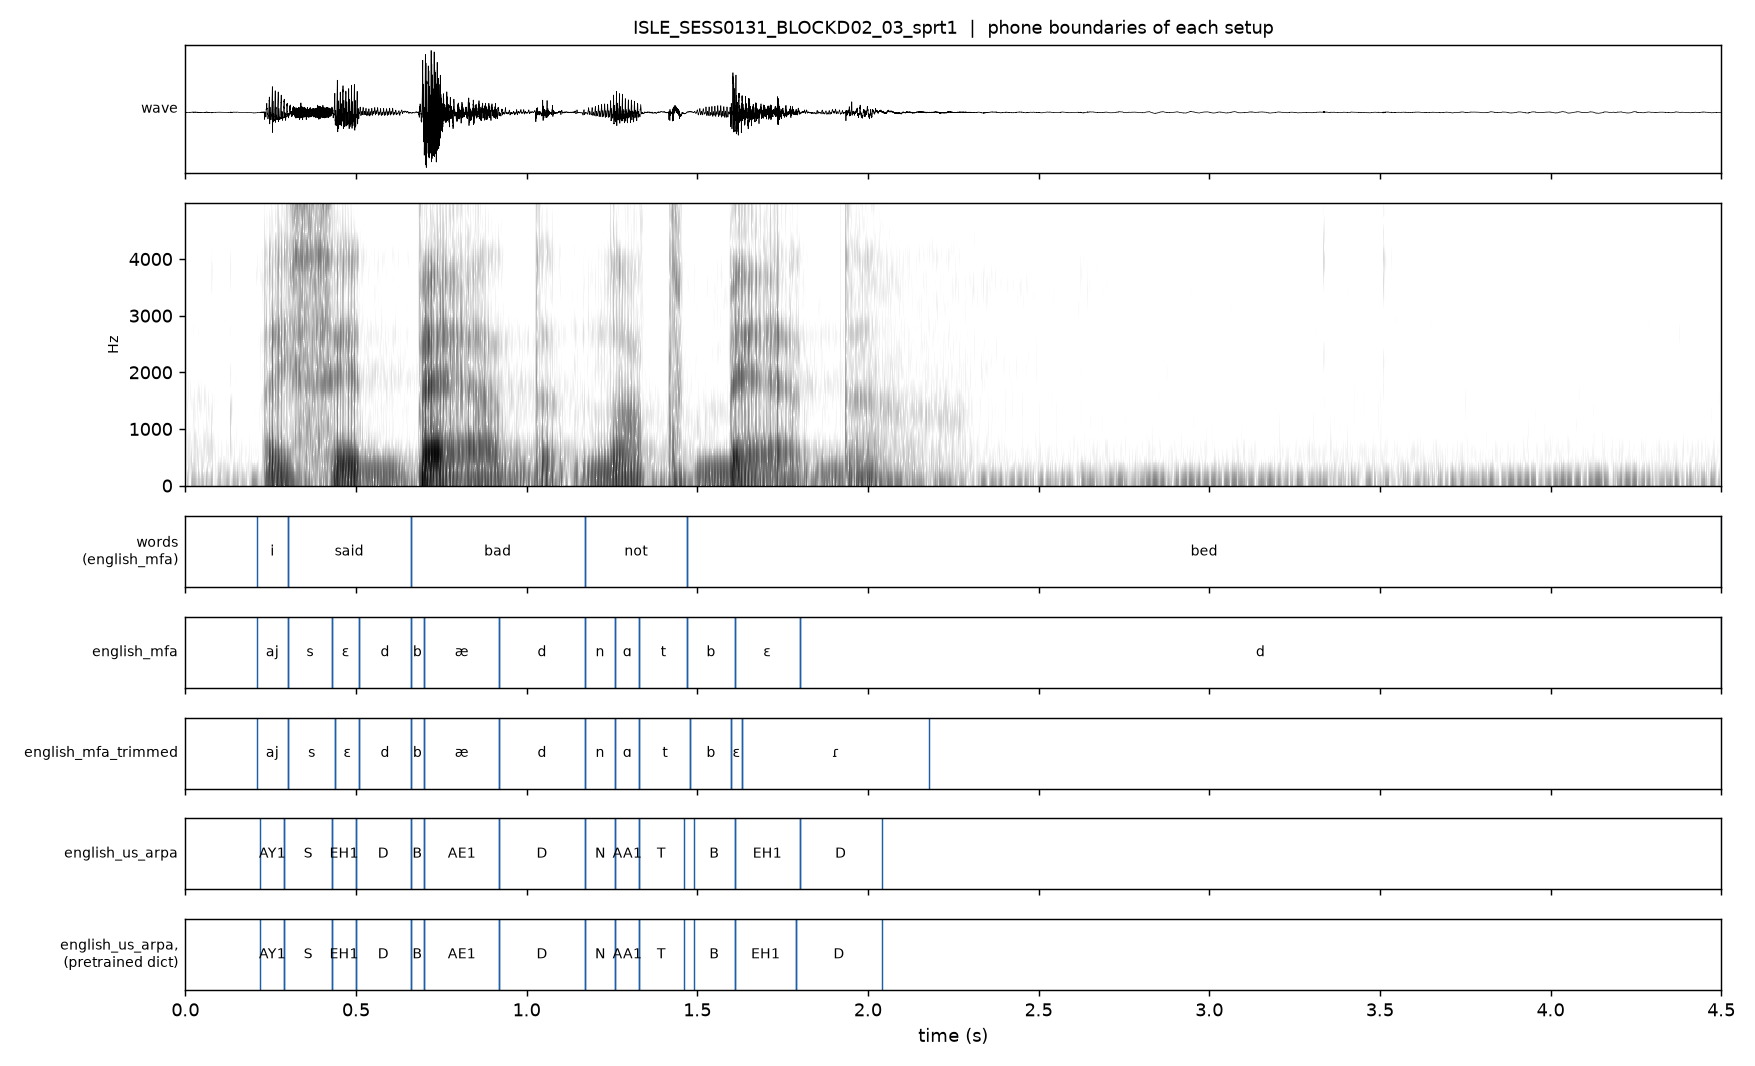
\includegraphics[width=\linewidth]{compare/ISLE_SESS0131_BLOCKD02_03_sprt1.png}
\caption{``I said BAD not BED'': waveform, spectrogram (Praat, 0--5\,kHz) and the phone tier of each setup.
\code{english\_us\_arpa} ends ``bed'' at the release of the /d/ (2.04\,s); \code{english\_mfa} stretches the /d/
to the end of the file (4.50\,s). On the trimmed file \code{english\_mfa} squeezes the vowel to 30\,ms and stretches
a flap [ɾ] to the new end.}
\label{fig:bed}
\end{figure}

\begin{figure}[!tbp]\centering
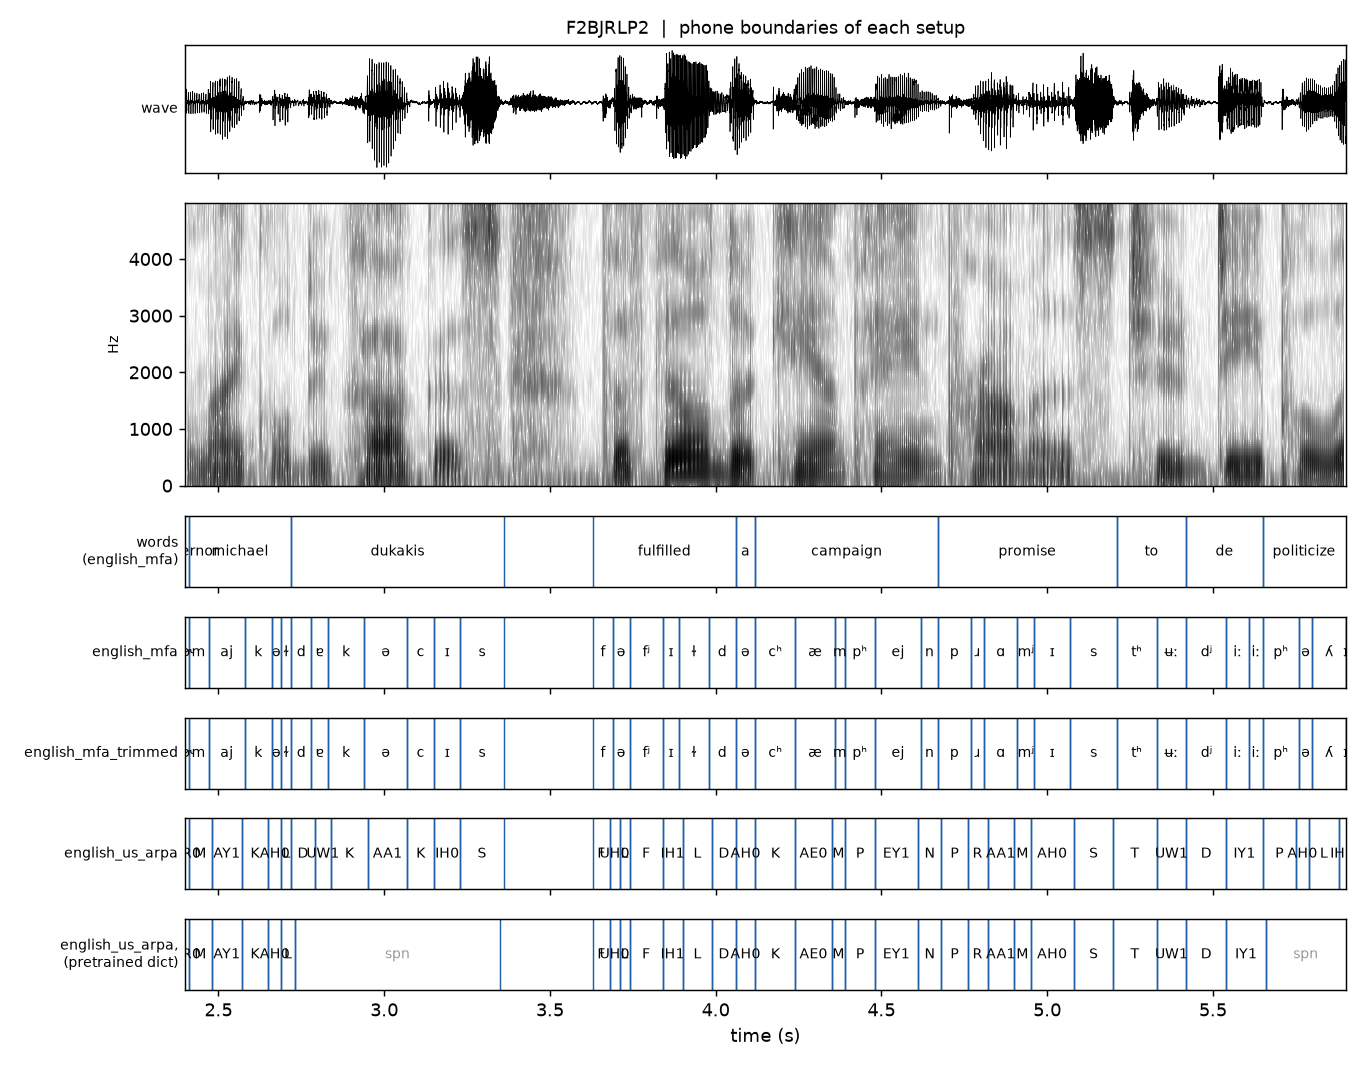
\includegraphics[width=\linewidth]{compare/F2BJRLP2.png}
\caption{News clip F2BJRLP2, 2.4--5.9\,s. With the pretrained dictionary, ``Dukakis'' and ``politicize'' are
unknown and get one \code{spn} interval each; with the G2P dictionary both models give them full phone
sequences, and the other boundaries hardly move.}
\label{fig:oov}
\end{figure}

\section{Observations}
\label{sec:obs}
\paragraph{How the boundaries line up.} Each word interval starts at its first phone and ends at its last, and
pauses are separate \code{sil} intervals. Every boundary falls on MFA's 10\,ms frame grid. The two models put half
of all 488 word boundaries within 10\,ms of each other, and 96\% within 50\,ms.

\paragraph{Trailing stops swallow the final silence (\code{english\_mfa}).} In ``bait'' and ``bed'', the last
words of two ISLE clips, \code{english\_mfa} labels 2.1\,s and 2.7\,s of silence as the final /t/ and /d/
(Figure~\ref{fig:bed}). The closure of a stop is itself near-silence, so the model can extend it instead of
switching to the silence model. The clip that ends in a vowel (``no'') comes out right, and
\code{english\_us\_arpa} gets all three right. This single error causes the largest disagreement in
Table~\ref{tab:agree}.

\paragraph{Cutting the silence caps the error but does not cure it.} The ``silence'' after these words is not
silent: a low hum sits 35--42\,dB below the speech peak. I cut each file 150\,ms after the last frame that comes
within 25\,dB of the peak, which keeps the start and therefore every earlier time (\code{english\_mfa\_trimmed}).
The largest disagreement with \code{english\_us\_arpa} falls from 2,460 to 250\,ms and the mean from 18.3 to
10.1\,ms. But \code{english\_mfa} still never places a final silence: it runs the last phone to the new end of
every short clip. In ``bed'' it now chooses the dictionary variant with a flap, [b ɛ ɾ], squeezes the vowel to
30\,ms and stretches the [ɾ] over 550\,ms. The length of the silence is therefore not the cause; the background
hum is the likelier one, which I did not test by denoising. For these clips \code{english\_us\_arpa} is the safer
model.

\paragraph{Unknown words.} Without G2P, each of the five unknown tokens becomes one \code{spn} interval
(Figure~\ref{fig:oov}). Its word boundaries still land in the right place, because the neighbouring words anchor
them, but the word gets no phones. With the G2P dictionary the same words get 4--9 phones, and no other boundary
moves by more than 20\,ms.

\paragraph{Skipped phones get squeezed, not deleted.} An aligner must place every phone the dictionary lists. When
the speaker drops or reduces one, it gets the shortest span the model allows. In the fast news reading, 82
ARPAbet phones (8\%) last 30\,ms or less, mostly /t/, /n/ and schwa; two schwas, in the ``double'' of
\emph{W B U R} and in \emph{will}, last a single 10\,ms frame. These are the deletions and reductions of fluent
speech, hidden behind a minimal duration.

\paragraph{Most pauses fall at punctuation, a third at phrase breaks without it.} The news clips have 21 pauses of
at least 100\,ms (\code{english\_us\_arpa}). Fourteen fall at punctuation; seven fall at phrase breaks with none, for
example after
the subject in ``Edward Hennessy \,|\, reaches the mandatory retirement age''. Five of the 19 punctuation marks
before the end of a clip got no pause: the reader ran through them.

\paragraph{The aligner trusts the transcript, not the speaker.} The ISLE speaker is a non-native learner saying
minimal pairs, and the aligner labels each vowel with the dictionary phone whatever he said. To see what he said, I
measured the first two formants at the middle of each target vowel with Praat (Burg method, 5,000\,Hz ceiling for a
male voice). Formants are resonances of the mouth: F1 rises the more open a vowel is, and F2 the further forward
the tongue sits.

\begin{table}[H]\centering\small
\caption{Target vowels in the minimal pairs (\code{english\_us\_arpa} boundaries).}
\label{tab:pairs}
\begin{tabular}{@{}llrrr@{}}
\toprule
Word & Aligned vowel & Duration & F1 & F2 \\
\midrule
white / bait & \code{AY1} / \code{EY1} & 150 / 200\,ms & 546 / 406\,Hz & 1,389 / 1,899\,Hz \\
new / no & \code{UW1} / \code{OW1} & 240 / 350\,ms & 308 / 363\,Hz & 1,338 / 847\,Hz \\
bad / bed & \code{AE1} / \code{EH1} & 220 / 190\,ms & 594 / 534\,Hz & 1,767 / 1,871\,Hz \\
\bottomrule
\end{tabular}
\end{table}

``White'' and ``bait'' differ by 140\,Hz in F1 and 510\,Hz in F2; ``new'' and ``no'' by 490\,Hz in F2. ``Bad'' and
``bed'' differ by only 60\,Hz in F1; in
the classic averages for American men (Peterson \& Barney, 1952: /æ/ 660\,Hz, /ɛ/ 530\,Hz) the gap is 130\,Hz. The
speaker may have produced the two vowels more alike than a native speaker would, a common difficulty for
learners, yet the alignment shows a perfect /æ/--/ɛ/ contrast.

\section{The aligner as a pronunciation checker}
\label{sec:pron}
The acoustic model can still judge which of two pronunciations fits the audio better, if the dictionary offers
both. For each target word I added a second pronunciation with its partner's vowel (\emph{bad} \code{B EH1 D},
\emph{bed} \code{B AE1 D}, \emph{white} \code{W EY1 T}, \ldots) and ran two tests with \code{english\_us\_arpa}
(\code{scripts/pronunciation\_check.py}):
\begin{itemize}
\item \textbf{Free choice.} One dictionary holds both pronunciations of every target word with equal prior, and the
TextGrid shows which one the aligner picked.
\item \textbf{Likelihood ratio.} Each clip is aligned three times: with the intended vowels, with the first target
word's vowel swapped, and with the second's swapped. The difference in total log-likelihood between a swapped and
the intended alignment is a log-likelihood ratio (LLR). The LLR turns positive when the partner's vowel explains
the audio better. Goodness-of-pronunciation scores rest on the same comparison; here MFA alone computes the
likelihoods.
\end{itemize}

\begin{figure}[!tbp]\centering
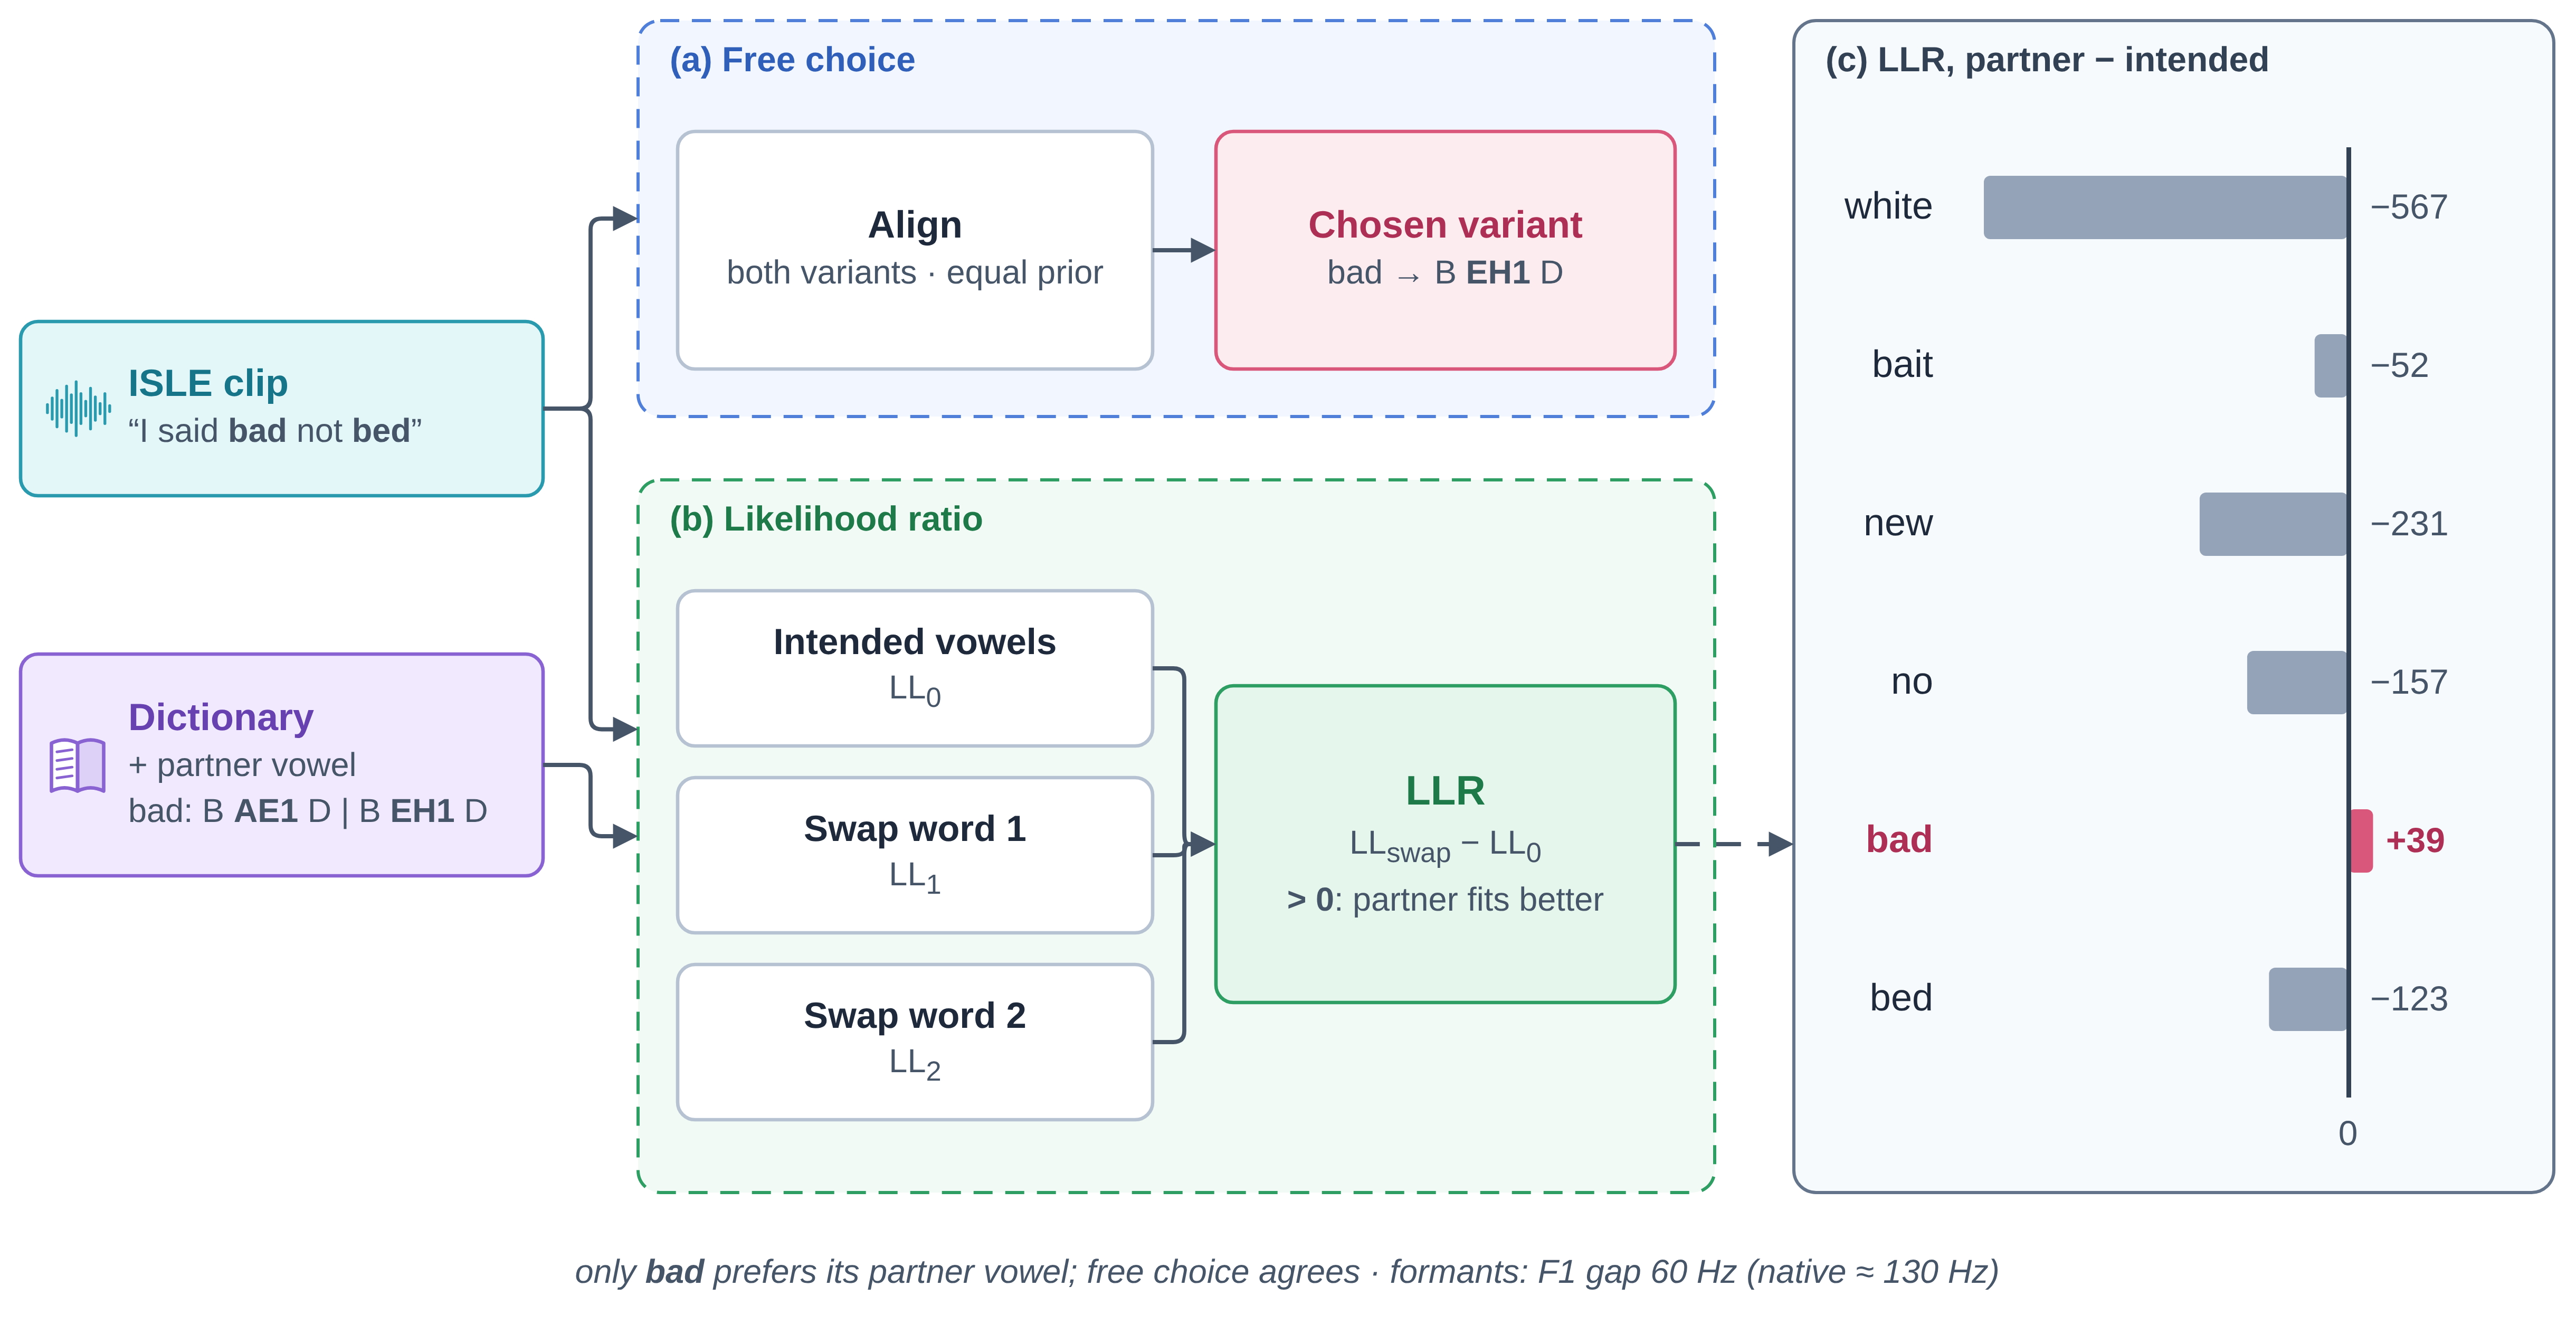
\includegraphics[width=0.92\linewidth]{fig3_pronunciation_check.png}
\caption{The pronunciation check. (a) Free choice: the aligner picks one of two pronunciations. (b) Likelihood
ratio: three alignments of each clip, with the intended vowels and with each target word's vowel swapped. (c) The
LLR of each target word; only ``bad'' scores above zero.}
\label{fig:pron}
\end{figure}

\begin{table}[H]\centering\small
\caption{Pronunciation check of the six target words.}
\label{tab:pron}
\begin{tabular}{@{}lllr@{}}
\toprule
Word & Intended & Aligner's free choice & LLR, partner $-$ intended \\
\midrule
white & \code{W AY1 T} & \code{W AY1 T} (intended) & $-$567 \\
bait & \code{B EY1 T} & \code{B EY1 T} (intended) & $-$52 \\
new & \code{N UW1} & \code{N UW1} (intended) & $-$231 \\
no & \code{N OW1} & \code{N OW1} (intended) & $-$157 \\
\textbf{bad} & \code{B AE1 D} & \textbf{\code{B EH1 D} (the vowel of ``bed'')} & \textbf{+39} \\
bed & \code{B EH1 D} & \code{B EH1 D} (intended) & $-$123 \\
\bottomrule
\end{tabular}
\end{table}

Both tests single out the same word (Figure~\ref{fig:pron}c). Given the choice, the aligner hears ``bad'' as \code{B EH1 D}, and ``bad'' is
the only word whose partner vowel fits better (LLR +39). The other five words prefer their own vowel, ``white''
most strongly ($-$567). The formants of Table~\ref{tab:pairs} point the same way: the F1 of ``bad'' (594\,Hz) lies
between the native /æ/ and /ɛ/ averages. Two independent measurements therefore agree that this speaker's ``bad''
moved towards ``bed'', the /æ/--/ɛ/ confusion common among learners of English. ``Bait'' prefers its own vowel only
weakly ($-$52), although its formants differ from those of ``white'' by 140 and 510\,Hz; one token cannot separate a speaker
effect from noise in the score. One recording per word makes all of this an observation about these clips, not a
diagnosis of the speaker. Repeated runs also differ slightly, because MFA adapts its model to each speaker
(fMLLR) from the run's own first-pass alignment: an earlier run gave +32 for ``bad'', with the same choices and
signs.

\section{Pipeline and extra credit}
\code{run\_pipeline.py} runs the whole process: corpus preparation, model download, G2P dictionaries, alignment
for each setup, figures and tables. The figures (\code{scripts/visualize.py}) use Praat's own engine through
parselmouth, and \code{scripts/analyze.py} writes the tables. The extra-credit items are a custom dictionary
(G2P), two acoustic models compared on the same data, and the automated pipeline. Beyond them, the pipeline tests
a remedy for the one systematic error it found (trailing-silence trimming) and uses the aligner as a pronunciation
checker (Section~\ref{sec:pron}). All TextGrids are in \code{outputs/textgrids/}; Praat
opens each one together with its \code{.wav} from \code{outputs/corpus/}.

\paragraph{Limitations.} There is no hand-made reference alignment, so I can measure agreement and spot errors
but not accuracy. \code{mfa validate} reports an unexplained error at its last step on this Windows install;
\code{mfa align} runs cleanly, so the pipeline uses it directly.

\end{document}
